\documentclass[compress]{beamer}

\mode<presentation>{
\usetheme{Sinica}
\usecolortheme{rose}
}
\usepackage{amsmath,amsfonts,amssymb}
\usepackage{CJKutf8}
\usepackage{colortbl}

%%% Template Setting

%% Font
\usefonttheme[onlylarge]{structuresmallcapsserif}
\usefonttheme[onlysmall]{structurebold}
\setbeamerfont{title}{shape=\itshape,family=\rmfamily}
\setbeamertemplate{frametitle}[default][center]


\title{ANTUSD: A Large Chinese Sentiment Dictionary }
\author{Shih-Ming Wang and Lun-Wei Ku}
\date[LREC 2016]{10th Language Resources and Evaluation Conference}
\subject{Computer Science}

\begin{document}
\beamertemplatenavigationsymbolsempty

\begin{frame}[plain]
    \titlepage
\end{frame}

\begin{frame}
    \frametitle{Outline}
    \tableofcontents % [pausesections]
\end{frame}
\section{Motivation}
    \begin{frame}{\secname}
        \begin{block}{Sentiment Dictionary}
            \begin{itemize}
                \item A building block of sentiment analysis \& opinion mining
                % \item A useful resource for both research and industrial communities
                \item Applied as markers or machine learning features
            \end{itemize}
        \end{block}
        \pause
        \begin{block}{Augmented NTU Sentiment Dictionary (ANTUSD)}
            \begin{itemize}
                \item Lack of Chinese resource
                \item Big \& complete
                \item Expert labeled sentiment \& machine predicted sentiment scores
            \end{itemize}
        \end{block}
    \end{frame}

\section{Corpus Building}
    \subsection{Related Corpora}
        \begin{frame}{\subsecname\ I}
            \begin{itemize}
                \item<1-> Words and labels were collected from several sentiment corpora (2006$\sim$2010)
            \end{itemize}
            \begin{block}<2->{Word-base, context free}
                \begin{itemize}
                    \item<2-> NTUSD
                        \begin{itemize}
                            \item<3-> A widely used Chinese sentiment dictionary
                            \item<3-> Labels: \textbf{POS} and \textbf{NEG} (2812/8276) 
                        \end{itemize}
                    \item<2-> ACIBiMA
                        \begin{itemize}
                            \item<4-> Chinese morphological structure on sentiment analysis
                            \item<4-> Labels: \textbf{POS}, \textbf{NEU}, \textbf{NEG}, \textbf{NONOP}, and \textbf{NOT}
                            \item<5-> \textbf{NONOP} indicates a non-emotion words
                            \item<5-> \textbf{NOT} indicates an incorrectly segmented word
                        \end{itemize}
                \end{itemize}
            \end{block}
            \note{Advanced Chinese Bi-Character Word Morphological Analyzer}
        \end{frame}

        \begin{frame}{\subsecname\ II}
            \begin{block}{Sentence-based, context dependent}
                \begin{itemize}
                    \item<1-> NTCIR Multilingual Opinion Analysis Test (MOAT) Dataset
                        \begin{itemize}
                            \item<2->  Dataset for international opinion analysis contest (6, 7 and 8th NTCIR)
                        \end{itemize}

                    \item<1-> Chinese Opinion Tree Bank
                        \begin{itemize}
                            \item<3-> Incorporate syntactic information (Chinese Treebank)\\ into sentiment analysis
                        \end{itemize}
                \end{itemize}
            \end{block}
            \begin{block}<4->{Properties}
                \begin{itemize}
                    \item Labels: \textbf{POS}, \textbf{NEU}, and \textbf{NEG}
                    \item Label process:  sentence $\rightarrow$ sentiment words
                    \item Each word might belong to conflicting labels
                    \item Context information not included in ANTUSD
                    \note{item Label count $\propto$ word frequency}
                \end{itemize}
            \end{block}
        \end{frame}

    \subsection{CopeOpi}
        \begin{frame}{\subsecname}
            \begin{block}{Machine predicted sentiment score}
                \begin{itemize}
                    \item CopeOpi: A Chinese opinion-analysis system
                    \item Sentiment scores of documents, sentences, words, and characters 
                    \item Polarity score of each character is calculated statistically
                    \item Word by summing up characters; sentence by summing up words...
                    \note{by counting the occurence of a word in documents labeled as positive or in documents labeled as negative}
                \end{itemize}
            \end{block}
        \end{frame}

    \subsection{Extended-HowNet (E-HowNet)}
        \begin{frame}{\subsecname}
            \begin{block}{E-HowNet}
                \begin{itemize}
                    \item A frame-based entity-relation model extended from HowNet
                    \item Define lexical senses (concepts) in a hierarchical manner
                    \item Now integrated with ANTUSD and covers 47.7\% words in ANTUSD
                \end{itemize}
            \end{block}
            \pause
            \begin{figure}
                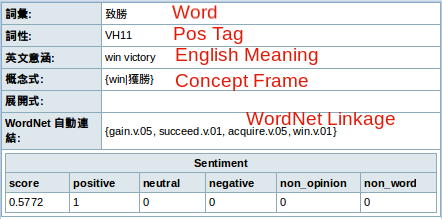
\includegraphics[height=.5\textheight]{e-hownet.png}
            \end{figure}
            \note{created by Dong etc. in 2006}
        \end{frame}

\section{Demonstrative Experiment}
    \begin{frame}{\secname}
        \begin{block}{Experiment Setting}
            \begin{itemize}
                \item Dataset: ANTUSD $\cap$ E-hownet, a total 12995 words
                \item Classifier: support vector machine (SVM) with linear kernel
                \item Average over 10-fold validation scores
            \end{itemize}
        \end{block}
        \pause
        \begin{block}{Three sentiment analysis tasks}
            \begin{itemize}
                \item Opinion extraction: identify opinion words \\ (\{\textbf{POS},\textbf{NEG}\}\ v.s. \textbf{NONOP})
                \item Polarity classification: classify opinion words (\textbf{POS} v.s. \textbf{NEG})
                \item Combined tasks (\textbf{POS}, \textbf{NEG}, \textbf{NONOP})
                \begin{itemize}
                    \item $P=\frac{correct(opinion) \cap correct(polarity)}{proposed(opinion)}$
                    \item $R=\frac{correct(opinion) \cap correct(polarity)}{gold(opinion)}$
                    \item $F-score = \frac{2PR}{P+R}$
                \end{itemize}
            \end{itemize}
        \end{block}
    \end{frame}

    \subsection{Preprocessing}
        \begin{frame}{\subsecname}
            \begin{block}{Extract single label for each word}
                \begin{enumerate}
                    \item \textbf{NOT}: Count(Not)$>$0
                    \item \textbf{NONOP}: Count(Non)$>$0  
                    \item \textbf{POS}: Count(Pos)$>$0 and Count(Neg)=0  
                    \item \textbf{NEG}: Count(Neg)$>$0 and Count(Pos)=0  
                    \item \textbf{NEU}: Count(Pos)=0, Count(Neg)=0 and Count(Neu)$>$0  
                \end{enumerate}
            \end{block}
            \pause
            \begin{itemize}
                \item Neutral words are dropped since there are only 16 of them
                \item Words not labeled are also dropped (e.g., Count(Pos)$>$0 and Count(Neg)$>$0)
            \end{itemize}
        \end{frame}

    \subsection{Features}
        \begin{frame}{\subsecname}
            \begin{block}{ANTUSD \& E-hownet}
                \begin{itemize}
                    \item CopeOpi score in ANTUSD
                    \item Synonym-Set index (SSI)
                        \begin{itemize}
                            \item Concept frame index of a word
                            \item Each word might belong to many concepts
                            \item Represented as a binary vector % each dimension corresponds to a concept
                        \end{itemize}
                    \end{itemize}
                \end{block}
            \pause
            \begin{block}{Word Embedding}
                \begin{itemize}
                    \item Corpus: LDC2009T14 (Chinese news)
                    \item Word vectors % low coverage, high quality
                    \item Summation of char vectors % high coverage, low quality   
                \end{itemize}
            \end{block}
        \end{frame}
    \subsection{Results}
        \begin{frame}{Opinion Extraction}
            \begin{columns}
                \begin{column}[T]{.5\textwidth}
                    \begin{itemize}
                        \item<1-> COP, SSI has lower precision
                            \begin{itemize}
                                \item opinion extraction  is more semantic-oriented
                                \item Many words contain single SSI
                            \end{itemize}
                        \item<2-> Character vectors lead to less precise semantic representation
                        \item<3-> Features are complemented; combined features leads to improvement
                    \end{itemize}
                \end{column}
                \begin{column}[T]{.6\textwidth}
                    \begin{table}
                    \small
                    \centering
                    \tabcolsep=0.1cm
                    \begin{tabular}{cccc}
                    \hline
                    Feature(s) & Precision & Recall & f-score \\ \hline
                    \only<1>{
                        COP        & \cellcolor{green}0.686     & 1.000  & 0.814   \\ \hline
                        SSI        & \cellcolor{green}0.693     & 0.993  & 0.816   \\ \hline
                        WV         & 0.784     & 0.936  & 0.854   \\ \hline
                        CV         & 0.765     & 0.919  & 0.835   \\ \hline
                        COP+SSI    & 0.740     & 0.914  & 0.818   \\ \hline
                        COP+WV     & 0.785     & 0.933  & 0.853   \\ \hline
                        COP+CV     & 0.764     & 0.917  & 0.833   \\ \hline
                        SSI+WV     & 0.789     & 0.937  & 0.856   \\ \hline
                        SSI+CV     & 0.772     & 0.920  & 0.840   \\ \hline
                        WV+CV      & 0.808     & 0.921  & 0.861   \\ \hline
                    }
                    \only<2>{
                        COP        & 0.686     & 1.000  & 0.814   \\ \hline
                        SSI        & 0.693     & 0.993  & 0.816   \\ \hline
                        WV         & 0.784     & 0.936  & \cellcolor{red}0.854   \\ \hline
                        CV         & 0.765     & 0.919  & \cellcolor{green}0.835   \\ \hline
                        COP+SSI    & 0.740     & 0.914  & 0.818   \\ \hline
                        COP+WV     & 0.785     & 0.933  & \cellcolor{red}0.853   \\ \hline
                        COP+CV     & 0.764     & 0.917  & \cellcolor{green}0.833   \\ \hline
                        SSI+WV     & 0.789     & 0.937  & \cellcolor{red}0.856   \\ \hline
                        SSI+CV     & 0.772     & 0.920  & \cellcolor{green}0.840   \\ \hline
                        WV+CV      & 0.808     & 0.921  & 0.861   \\ \hline
                    }
                    \only<3>{
                        COP        & 0.686     & 1.000  & \cellcolor{green!50}0.814   \\ \hline
                        SSI        & 0.693     & 0.993  & \cellcolor{cyan!50}0.816   \\ \hline
                        WV         & 0.784     & 0.936  & \cellcolor{blue!50}0.854   \\ \hline
                        CV         & 0.765     & 0.919  & \cellcolor{blue!50}0.835   \\ \hline
                        COP+SSI    & 0.740     & 0.914  & \cellcolor{green}0.818   \\ \hline
                        COP+WV     & 0.785     & 0.933  & \cellcolor{green}0.853   \\ \hline
                        COP+CV     & 0.764     & 0.917  & \cellcolor{green}0.833   \\ \hline
                        SSI+WV     & 0.789     & 0.937  & \cellcolor{cyan}0.856   \\ \hline
                        SSI+CV     & 0.772     & 0.920  & \cellcolor{cyan}0.840   \\ \hline
                        WV+CV      & 0.808     & 0.921  & \cellcolor{blue!80}0.861   \\ \hline
                    }
                    \end{tabular}
                    \end{table}
                \end{column}
            \end{columns}
        \end{frame}
        \begin{frame}{Polarity Classification}
            \begin{columns}
                \begin{column}[T]{.5\textwidth}
                    \begin{itemize}
                        \item<1-> COP leads to a significant better result, reflecting is sentiment-oriented nature
                        \item<2-> Combining COP \& other features still leads to improvement
                        \item<3-> Combining word vectors and SSI also leads to improvement % which meancs SSI can be used to increas the quality of word embedding
                    \end{itemize}
                \end{column}
                \begin{column}[T]{.6\textwidth}
                    \begin{table}
                    \small
                    \centering
                    \tabcolsep=0.1cm
                    \begin{tabular}{cccc}
                    \hline
                    Feature(s) & POS f1 & NEG f1 & Average f1 \\ \hline
                    \only<1>{
                        COP        & 0.973  & 0.976  & \cellcolor{red}0.974      \\ \hline
                        SSI        & 0.792  & 0.842  & 0.817      \\ \hline
                        WV         & 0.870  & 0.895  & 0.882      \\ \hline
                        CV         & 0.829  & 0.851  & 0.840      \\ \hline
                        COP+SSI    & 0.979  & 0.982  & 0.980      \\ \hline
                        COP+WV     & 0.981  & 0.984  & 0.982      \\ \hline
                        COP+CV     & 0.967  & 0.972  & 0.970      \\ \hline
                        SSI+WV     & 0.898  & 0.915  & 0.907      \\ \hline
                        SSI+CV     & 0.868  & 0.886  & 0.877      \\ \hline
                        WV+CV      & 0.899  & 0.916  & 0.908      \\ \hline
                    }
                    \only<2>{
                        COP        & 0.973  & 0.976  & \cellcolor{green}0.974      \\ \hline
                        SSI        & 0.792  & 0.842  & 0.817      \\ \hline
                        WV         & 0.870  & 0.895  & 0.882      \\ \hline
                        CV         & 0.829  & 0.851  & 0.840      \\ \hline
                        COP+SSI    & 0.979  & 0.982  & \cellcolor{red}0.980      \\ \hline
                        COP+WV     & 0.981  & 0.984  & \cellcolor{red}0.982      \\ \hline
                        COP+CV     & 0.967  & 0.972  & 0.970      \\ \hline
                        SSI+WV     & 0.898  & 0.915  & 0.907      \\ \hline
                        SSI+CV     & 0.868  & 0.886  & 0.877      \\ \hline
                        WV+CV      & 0.899  & 0.916  & 0.908      \\ \hline
                    }
                    \only<3>{
                        COP        & 0.973  & 0.976  & 0.974      \\ \hline
                        SSI        & 0.792  & 0.842  & \cellcolor{green}0.817      \\ \hline
                        WV         & 0.870  & 0.895  & \cellcolor{green}0.882      \\ \hline
                        CV         & 0.829  & 0.851  & 0.840      \\ \hline
                        COP+SSI    & 0.979  & 0.982  & 0.980      \\ \hline
                        COP+WV     & 0.981  & 0.984  & 0.982      \\ \hline
                        COP+CV     & 0.967  & 0.972  & 0.970      \\ \hline
                        SSI+WV     & 0.898  & 0.915  & \cellcolor{red}0.907      \\ \hline
                        SSI+CV     & 0.868  & 0.886  & 0.877      \\ \hline
                        WV+CV      & 0.899  & 0.916  & 0.908      \\ \hline
                    }
                    \end{tabular}
                    \end{table}
                \end{column}
            \end{columns}
        \end{frame}
        \begin{frame}{Combined Task}
            \begin{columns}
                \begin{column}[T]{.5\textwidth}
                    \begin{itemize}
                        \item<1-> COP outperforms the others
                        \item<2-> Both the numerator of precision and recall are affected by COP’s better polarity classification ability
                        \item<2-> Only the denominator of precision is affected by COP's worse opinion  extraction  ability
                        \item<3> WV+CV outperforms WV due to coverage issue
                    \end{itemize}
                \end{column}
                \begin{column}[T]{.6\textwidth}
                    \only<2>{
                    \begin{block}{Precision \& Recall}
                        $P=\frac{correct(opinion) \cap correct(polarity)}{proposed(opinioopinionn)}$\\
                        $R=\frac{correct(opinion) \cap correct(polarity)}{gold(opinioopinionn)}$
                    \end{block}
                    }
                    \begin{table}
                    \small
                    \centering
                    \tabcolsep=0.1cm
                    \begin{tabular}{cccc}
                    \hline
                    Feature(s) & Precision & Recall & f-score \\ \hline
                    \only<1,2>{
                        COP        & 0.912     & 0.927  & \cellcolor{red}0.920   \\ \hline
                        SSI        & 0.706     & 0.679  & 0.692   \\ \hline
                        WV         & 0.737     & 0.767  & 0.752   \\ \hline
                        CV         & 0.689     & 0.721  & 0.705   \\ \hline
                        COP+SSI    & 0.864     & 0.945  & 0.903   \\ \hline
                        COP+WV     & 0.850     & 0.902  & 0.875   \\ \hline
                        COP+CV     & 0.840     & 0.869  & 0.854   \\ \hline
                        SSI+WV     & 0.764     & 0.796  & 0.779   \\ \hline
                        SSI+CV     & 0.732     & 0.755  & 0.743   \\ \hline
                        WV+CV      & 0.764     & 0.813  & 0.787   \\ \hline
                    }
                    \only<3>{
                        COP        & 0.912     & 0.927  & 0.920   \\ \hline
                        SSI        & 0.706     & 0.679  & 0.692   \\ \hline
                        WV         & 0.737     & 0.767  & \cellcolor{green}0.752   \\ \hline
                        CV         & 0.689     & 0.721  & \cellcolor{green}0.705   \\ \hline
                        COP+SSI    & 0.864     & 0.945  & 0.903   \\ \hline
                        COP+WV     & 0.850     & 0.902  & 0.875   \\ \hline
                        COP+CV     & 0.840     & 0.869  & 0.854   \\ \hline
                        SSI+WV     & 0.764     & 0.796  & 0.779   \\ \hline
                        SSI+CV     & 0.732     & 0.755  & 0.743   \\ \hline
                        WV+CV      & 0.764     & 0.813  & \cellcolor{red}0.787   \\ \hline
                    }
                    \end{tabular}
                    \end{table}
                \end{column}
            \end{columns}
        \end{frame}

\section{Conclusion}
    \begin{frame}{\secname}
        \begin{itemize}
            \item A so far the largest Chinese sentiment dictionary
            \item Manually sentiment labels \& machine estimated sentiment scores 
            \item Three experiments were conducted to demonstrate the usage of ANTUSD
        \end{itemize}
    \end{frame}

    \begin{frame}{}
        \begin{center}
            \huge
            Q \& A
        \end{center}
    \end{frame}
\end{document}
